\chapter{Recherche bibliographique}

\section{Démarche de recherche}

\paragraph{}

Pour répondre à notre problématique de {\bf{détection d'anomalies dans les séries temporelles, dans un cadre non supervisé}}, nous avons consulté plus de 70 ressources sur les nombreux thèmes associés à notre sujet, avec deux objectifs : monter en compétence sur des notions que nous ne connaissions pas encore suffisamment et réaliser un état de l'art des méthodes susceptibles de répondre à la problématique. (~\ref{fig: bibnat})


\begin{figure}[!ht]
\begin{center}
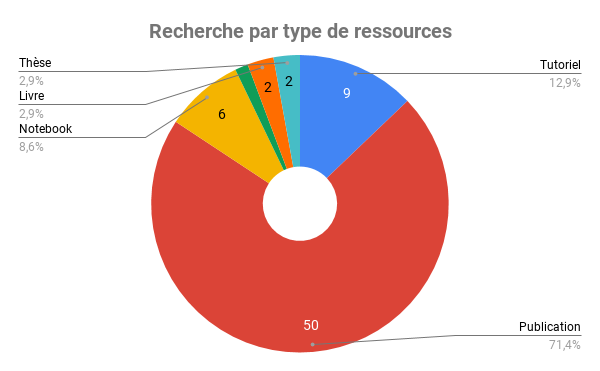
\includegraphics[scale=0.5]{rapport/images/Ch3_RechercheParTypeRessources.png}
\end{center}
\caption{Recherche par type de documents}
\label{fig: bibnat}
\end{figure}
\FloatBarrier


\begin{figure}[!ht]
\begin{center}
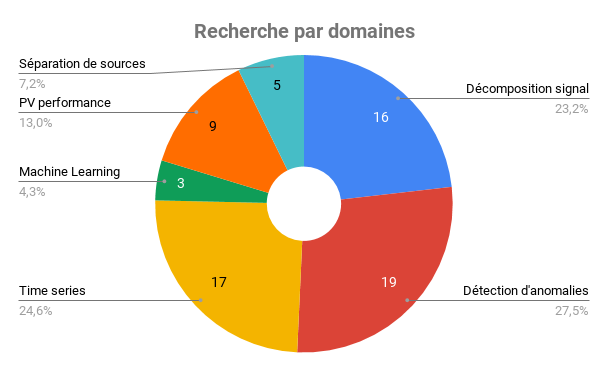
\includegraphics[scale=0.5]{rapport/images/Ch3_RechercheParDomaines.png}
\end{center}
\caption{Recherche par domaine}
\label{fig: bibdo}
\end{figure}

\paragraph{Notes sur la notion d'anomalie}
\paragraph{}
Puisque l'on est amené à détecter des anomalies, il nous paraît pertinent de préciser ce que recouvre cette notion. Dans le cadre général, la détection d'anomalie consiste à trouver des motifs non usuels dans les données. Ces anomalies sont différentes du bruit et sont généralement catégorisées de la façon suivante :

\begin{enumerate}
\item Les anomalies ponctuelles (un point dont la valeur excède la gamme de valeurs de la distribution des données)
\item Les anomalies contextuelles (des valeurs non usuelles pour le contexte donné)
\item Les anomalies collectives (une gamme de valeurs non usuelles)
\end{enumerate}

Dans le cas des signaux électriques mesurés au niveau des onduleurs, il est nécessaire de distinguer les anomalies causées par la défaillance d'équipements composant les panneaux solaires des anomalies causées par un phénomène extérieur. En effet les changements de signaux électriques indépendants du fonctionnement normal doivent aussi être identifiés afin de ne pas être considérés comme une défaillance du système. Ces variations peuvent provenir des perturbations météorologiques, de phénomènes contextuelles tels la pousse de végétation ou encore salissure du panneaux.

Pour pouvoir répondre à la problématique de ce projet, nous avons restreint notre analyse aux sujets traitant de détection d'anomalie dans les séries temporelles à caractère non permanent.

%\paragraph{}
%Dans notre cas, l'anomalie serait due à une panne d'un onduleur.
% A bien montrer, qu'un changement (sous-performance d'un onduleur) due à une cause météorologique n'est pas une anomalie à proprement parlé

\section{Panorama des méthodes}
\paragraph{}
Des recherches ont été réalisées au sein de plusieurs laboratoires comme le NREL (National Renewable Energy Laboratory) pour détecter les défaillances/pannes des composants constituant les panneaux photovoltaiques (PV). D'après \cite{FaultSolarPanel} les modèles utilisés pour traiter ce type de problématique sont essentiellement :
\begin{itemize}
    \item Des modèles d'apprentissage automatique(31\%)
    \item Des modèles de traitement du signal électrique (9 \%)
    \item Des modèles à base d'analyses statistiques (14 \% )
\end{itemize}
Cependant, dans la majorité de ces publications, il s'agit d'un cadre supervisé où les différentes signatures électriques sont connues ou simulées.

\paragraph{}
Nous avons donc élargi nos recherche pour nous focaliser sur les études traitant de séries temporelles transientes dans un cadre non supervisé.

%\subsection{Différentes méthodes répertoriées}
Au travers de nos recherches, nous avons identifié plusieurs types de méthodes qui pourraient s'adapter à notre problématique et que l'on peut répartir schématiquement en trois familles, comme présenté dans le tableau \ref{tab:Methods} avec les principaux papiers qui leur sont associés.
%\begin{enumerate}
%    \item Méthodes en deux temps  (Extraction de caractéristiques suivie d'un algorithme d'apprentissage)
%    \item Apprentissage du signal 
%    \item Algorithmes prédictifs 
%\end{enumerate}
\paragraph{}
\paragraph{}
\begin{table}[h!]
\resizebox{15cm}{!}{
\begin{center}
   \begin{tabular}{ || l  || l  ||  l || }
     \hline
      \bf{Famille d'ensemble} & \bf{Méthodes} & \bf{Domaine d'application}\\
     \hline
       Décomposition + classification & Ondelettes, EMD/LMD + ML & ECG  \cite{INCE} /Satellites \cite{BClementine}   \\ \hline
         & Séparation de sources (NMF, ICA) & Musique, vidéo, EEG, consommation électrique \cite{JialiM}  \\ \hline
        Apprentissage du signal normal  &  Réseau de neurones, LSTM ou Auto-encodeur  & Défaillance réseau électrique \cite{ferhartUc}, \cite{MalhotraP}  \\ \hline
        Algorithmes prédictifs & Ex. ARIMA   & Monitoring \cite{MMostafa} \\ \hline
     \hline
   \end{tabular}
 \end{center}}
\caption{Familles de méthodes identifiées}
\label{tab:Methods}
\end{table}


\paragraph{}
La première famille de méthodes est très largement utilisée par la communauté scientifique et nous semble particulièrement adaptée au projet. Elle consiste en deux phases : d'abord une décomposition du signal pour extraire des caractéristiques (via des techniques qui varient selon les cas), puis une utilisation de ces caractéristiques dans des algorithmes d'apprentissage statistique (clustering, réseaux de neurone, ..). %Les signaux normaux et anormaux sont donc identifiés.
\paragraph{}
Les cas d'applications de ces méthodes sont très variés. Ils s'étendent du domaine médical à l'ingénierie en passant par l'analyse des défaillances électriques. Il existe pléthore de recherches appliquées à la détection d'anomalies pour les maladies cardiaques, par exemple. Luz et al. \cite{Luz} passe en revue les différentes techniques utilisées (algorithmes génétiques, réseaux de neurones) appliquées au traitement des électrocardiogrammes, parmi lesquelles :
\begin{enumerate}
    \item Séparation de sources (NMF, ICA) %\cite{Chawla}
    \item Clustering direct sur des points échantillonnés sur la courbe %\cite{Ozbay}
    \item Generalized Discriminant Analysis 
    \item Wavelet transform et classification sur les caractéristiques extraites \cite{Guler}, \cite{BClementine}
\end{enumerate}
Les spécialistes de ce domaine considèrent que la technique de décomposition en ondelettes donne les meilleurs résultats pour extraire des caractéristiques pertinentes des électrocardiogrammes. Néanmoins, il est important de s'interroger sur le choix de l'ondelette mère choisie, qui a un impact important sur les résultats finaux.
\paragraph{}
Les caractéristiques utilisées pour nourrir l'algorithme de classification varient aussi sensiblement suivant les publications.

Dans l'étude de \cite{Guler}, sont utilisées par exemple différentes métriques statistiques (moyenne, variance etc..) décrivant les signaux reconstruits à chaque niveau de décomposition, utilisées par la suite comme entrée dans un réseau de neurones. 
L'étude \cite{INCE}, utilise quant à elle, les coefficients d'ondelettes projetés dans un espace réduit grâce à une PCA (Principal Component Analysis) comme données d'entrée de l'algorithme de réseau de neurones.

\paragraph{}
Les ingénieurs du domaine spatiale s'intéressent également à ce type de problématique. La thèse de BARREYRE, Clementine \cite{BClementine}, détaille cette approche dans le cas des données fonctionnelles émises par les satellites (télémesures).
Dans cette étude, C.Barreyre nous expose une méthodologie similaire et extrait du signal des coefficients d'ondelettes qui sont des données d'entrée pour des algorithmes classiques de détection d'anomalie comme  One-Class SVM, LOF (Local Outlier Factor) et différentes méthodes de clustering.


\section{Description de 3 méthodes sélectionnées}
À partir du panorama précédent, nous avons sélectionné trois méthodes qui nous semblaient les plus pertinentes pour notre problématique, à savoir :

\begin{enumerate}
    \item La décomposition par ondelettes et apprentissage statistique
    \item La décomposition par méthodes adaptatives et recherche de similarités
    \item La séparation de sources par factorisation de matrices positives (NMF)
\end{enumerate}

%Nous avons choisie de décomposer le signal en ondelettes...
\subsection{Méthode 1 : La décomposition par ondelettes et apprentissage statistique }
%\section{Décomposition du signal }
%\subsection{Décomposition en ondelettes}
\subsubsection{Motivation}
\paragraph{}
Différentes méthodes de décomposition existent.
La plus connue et utilisée, est la transformée de Fourier. Cette dernière permet de filtrer le signal à différentes fréquences temporelles. Elle informe donc sur le contenu fréquentiel du signal.
Cependant elle possède une limitation majeure dans la connaissance du comportement local d'une fonction.
Ce défaut a été observé par D.Gabor qui a réussi à pallier à cette inconvénient en utilisant la STFT (short-time Fourier transform). Seulement la résolution temporelle restait insuffisante.
Elle n'est donc pas adéquate pour l'étude de signaux dans un régime transitoire. ~\cite{GaoR}.
\paragraph{}
La décomposition en ondelettes permet de pallier à ce défaut.
Elle prend en compte la variabilité fréquentielle de la fonction. 
Elle donne donc une \emph{représentation temps-fréquence d'un signal} ~\cite{JBigot}.
et permet donc de fournir une localisation temporelle.
Du fait du caractère transient de notre signal, un de nos choix s'est donc porté sur la transformée en ondelette.

\subsubsection{Théorie}
Cette partie contient les fondements généraux de la décomposition en ondelette.

La transformée en ondelettes ~\cite{JBigot} continue d'une fonction $f  \in L^{2}(\R)$ au point $x \in \R $
et à l'échelle $ s>0 $ est définie par  :
\begin{equation}
W_{f}(x,s) = <f,\Psi_{x,s}> = \int^{+\infty}_{- \infty} \frac{1}{\sqrt{s}}f(t)\Psi(\frac{t-x}{s})dt
\end{equation} 
Une transformée en ondelettes peut s'écrire sous la forme d'un filtrage par convolution :
\begin{equation}
W_{f}(x,s) = f * \psi^{*}_{s}(x)
\end{equation}
avec  $\psi^{*}_{s}(x) = \frac{1}{\sqrt{s}} \psi(\frac{-t}{s})$

\paragraph{}
%a transformée en ondelette satisfait les propriétés de conservation de l'énergie du signal.
L'ondelette choisie doit avoir :
\begin{enumerate}
\item un support compact pour obtenir une localisation dans l'espace
\item une moyenne égale à 0
\end{enumerate}
\paragraph{}
Il existe plusieurs types d'ondelettes :
\begin{enumerate}
\item Haar
\item Mexican hat
\item Morlet
\item Daubechie

\end{enumerate}

On utilisera l'ondelette Daubechie qui est la plus souvent utilisée d'après la littérature.

\paragraph{}
La transformée en ondelette permet de représenter une fonction comme une combinaison linéaire de fonctions de bases d'ondelettes.

Elle permet de réprésenter une fonction dans une \emph{représentation multirésolution d'ondelettes}. Cela consiste à une séquences d'espaces fermées $V_{m}$ de $ L^{2}(\R)$ où
$L^{2}(\R)$ est un espace d'Hilbert de toutes les fonctions au carré intégrables.
Ces espaces caractérisent le comportement d'une fonction à l'échelle $2^{m}$ échantillons par unité de longueurs.


\paragraph{}
Les coefficients de la transformée en ondelettes sont calculées par
\begin{equation}
W_{f}(x,s) = f * \psi^{*}_{s}(x)
\end{equation}


La fonction que l'on souhaite décomposer est réalisée de la façon suivante :
\begin{equation}
f(x)= \sum^{2j0-1}_{k=0} \alpha_{0,k}\phi_{j0,k} +\sum \sum^{2j0-1}_{k=0}\beta_{j,k}\psi_{j,k}
\end{equation}
%\alpha_{0,k}\phi_{j0,k} +\sum \sum^{2j0-1}_{k=0}\beta_{j,k}\psi_{j,k}
\begin{equation}
f(x) =f_{J0}(x) +\sum_{j>j0} D_{j}(x)
\end{equation}

Les coefficients d'ondelettes sont calculées de la manière suivante :
avec le coefficient d'échelle :
\begin{equation}
\alpha = \int^{1}_{0}f(x)\phi(x)dx
\end{equation}
et le coefficient de détail :
\begin{equation}
\beta_{j,k} = \int^{1}_{0}f(x)\psi(x)dx
\end{equation}

$\phi(x)$ est appelé l'ondelette mère
et $\psi(x) $ est l'ondelette père .

Pour une ondelette de Haar (ou Daubechie) , elles sont de la forme 



\begin{equation}
\psi(x) = \left\{
    \begin{array}{ll}
        -1 & \mbox{si } \{x\} \in [0,1/2] \\
        1 & \mbox{si } \{x\} \in ]1/2,1]
    \end{array}
\right.
\end{equation}


\begin{equation}
\phi(x) = \left\{
    \begin{array}{ll}
        1 & \mbox{si } \{x\} \in [0,1[ \\
        0 & \mbox{sinon.} 
     \end{array}
\right.
\end{equation}


\subsubsection{Application}

Dans notre cas, la décomposition en ondelette sera utilisée comme un moyen d'extraire du signal des caractéristiques pour ensuite détecter des anomalies.
Cependant, ce type de décomposition possède des limitations. 
Elles manquent de flexibilité aux différents signaux et doivent adapter les familles d'ondelettes au signal.

\subsection{Méthode 2 : Décomposition adaptative et recherche de similarités}

%\subsection{Décomposition en EMD et LMD}
% A mettre ce qu'elle apporte de plus par rapport aux ondelettes
\subsubsection{Motivation}
\paragraph{}
%A mettre avant les méthodes d'ondelettes
%Les méthodes numériques de traitements de signaux non-linéaires et non-stationnaires sont l'objet de nombreuses publications. Comme l'ont souligné Nicolas Di Palma, Alain Batailly et Mathias Legrand \cite{NAM}, les transformées de Fourrier appréhendent avec difficulté les comportements locaux et sont limitées par leur résolution temporelle.

%Les transformées en ondelettes manquent de flexibilité aux différents signaux et doivent adapter les /familles d'ondelettes au signal.

Les méthodes adaptatives approchent la décomposition du signal sous la somme de signaux calculés à partir des moyennes locales. Les méthodes avec le plus de publications et application sont l'EMD (décomposition en modes empiriques) et la LMD (décomposition en moyenne locale). Toutes deux s'affranchissent des problèmes d'adaptabilité rencontrés avec les ondelettes. 


\subsubsection{Théorie}
De façon itérative, les méthodes adaptatives extraient un large spectre de composantes de la plus oscillante jusqu'à obtenir un résidu presque monotone. Reposant principalement sur des considérations intuitives, de nombreuses formulations théoriques ont vu le jour pour définir les méthodes adaptatives. Un consensus semble rassembler la communauté autour de la formulation de NE Huang \cite{EMD-maths}. Le signal $x$ se décompose de la façon suivante:  
\begin{equation}
x(t) = \sum_{k=1}^{n}{h_k(t)} + r(t)
\end{equation}
Le signal $x(t)$ correspond à la somme des composantes $h_k(t)$ respectant les règles fixées par la méthode adaptative choisie et du résidu final considéré comme quasi nul. Seul les composantes vérifiant les propriétés d'un mode intrinsèque sont retenus comme décomposition du signal, à savoir \cite{NAM}: 
\begin{enumerate}
\item La différence entre le nombre d’extrema et le nombre de zéros de la fonction doit être nulle ou au plus égale à 1. 
\item La valeur moyenne de la somme des enveloppes supérieures (définies par les maxima) et inférieures (définies par les minima de la fonction) doit être nulle.
\end{enumerate}


\subsubsection{Spécificité de l'EMD}

La construction des modes intrinsèques, dans le cadre de l'EMD, se calcule en enlevant de façon itérative la moyenne de l'enveloppe supérieure et de l'enveloppe inférieure au signal restant à décomposer.  

On peut écrire $h_k$ sous la forme :
\begin{equation}
    h_{k+1}(t) = r_k(t)  - \sum_{i=1}^{n} \frac{e^{sup}_i(t) + e^{inf}_i(t)}{2}
\end{equation}
 avec $r_{k+1}(t)=r_k(t)-h_{k+1}(t)$
 \paragraph{}
 
\begin{figure}[!h]
    \begin{center}
        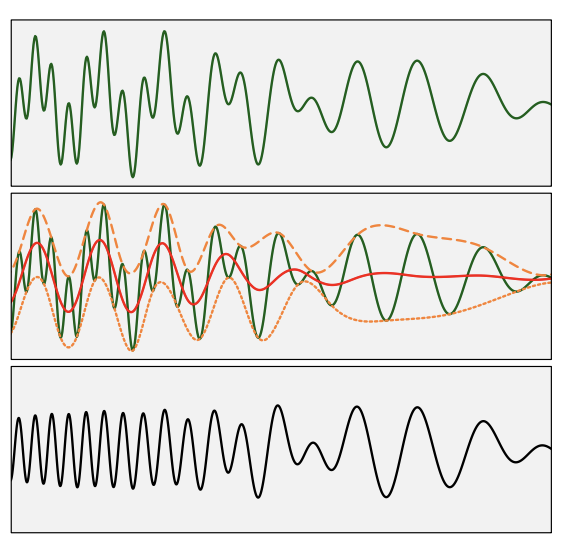
\includegraphics[scale=0.8]{rapport/images/Ch3_EMD.png}
    \end{center}
    \caption{Itération du processus de décomposition par EMD \cite{NAM}}
    \label{fig:EMD}
\end{figure}

La figure ~\ref{fig:EMD} illustre une itération simplifiée de la décomposition du signal. Le signal $r_k(t)$ est représenté en vert. Il s'agit du signal restant après soustraction des décompositions identifiées. le signal en rouge correspond à la moyenne des enveloppes supérieures et inférieures (en orange). Le résidu (en noir) recalculé à chaque itération correspond à la différence entre le signal vert et le signal rouge.


\subsubsection{Spécificité de la LMD}
\paragraph{}
La LMD construit ses composantes à partir des moyennes locales et des magnitudes locales des enveloppes. Les valeurs sont lissées à l'aide de moyennes glissantes.
\paragraph{}
On peut formuler $h_k$ de la façon suivante:
\begin{equation}
    h_{k+1}(t) = \frac{r_k(t) - \sum_{i=1}^{n}{m_i(t) \prod_{j=0}^{i}a_j(t) } }{\prod_{i=1}^{n}a_i(t)}
\end{equation}
avec $r_{k+1}(t)=r_k(t)-h_{k+1}(t)$ et $a_{j=0}(t) = 1$ où $a(t)$ correspond aux magnitudes locales et $m(t)$ les moyennes locales.
\begin{figure}[!h]
\begin{center} 
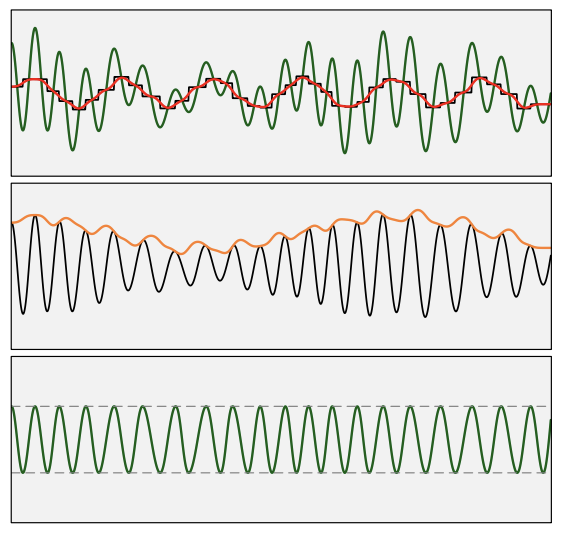
\includegraphics[scale=0.8]{rapport/images/Ch3_LMD.png} \end{center}
\caption{Itération du processus de décomposition par LMD \cite{NAM}}
\label{fig:LMD}
\end{figure}
\paragraph{}
La figure \ref{fig:LMD} illustre la construction d'une décomposition du signal par LMD. Le signal $r_k(t)$ apparaît dans la première partie de la figure en vert et l'on peut également voir en rouge le calcul des moyennes locales. La seconde partie présente en noir la différence de $r_k(t)$ et $m(t)$ et la construction de l'enveloppe $a(t)$ en orange. 
La dernière partie présente le signal décomposé en vert.
\subsubsection{Application}
Les méthodes adaptatives ont fait leurs preuves dans divers domaines tels que la santé ou les systèmes industriels. En effet, la LMD propose des analyses pertinentes dans le cas d'étude d'encéphalogrammes \cite{test_LMD} et, l'EMD à permis d'extraire les bruits et de reconstruire les signaux de systèmes mécaniques \cite{MFD}.

\subsection{Méthode 3 : Séparation de sources par factorisation NMF}
\subsubsection{Motivation}
La factorisation NMF existe depuis plus de trente ans et propose une représentation par parties, non supervisée, des données. Elle s'appuie sur une décomposition de la matrice des données V en un produit de deux matrices de variables explicatives W et de coefficients d'activation H :

\begin{figure}[!ht]
\begin{center}
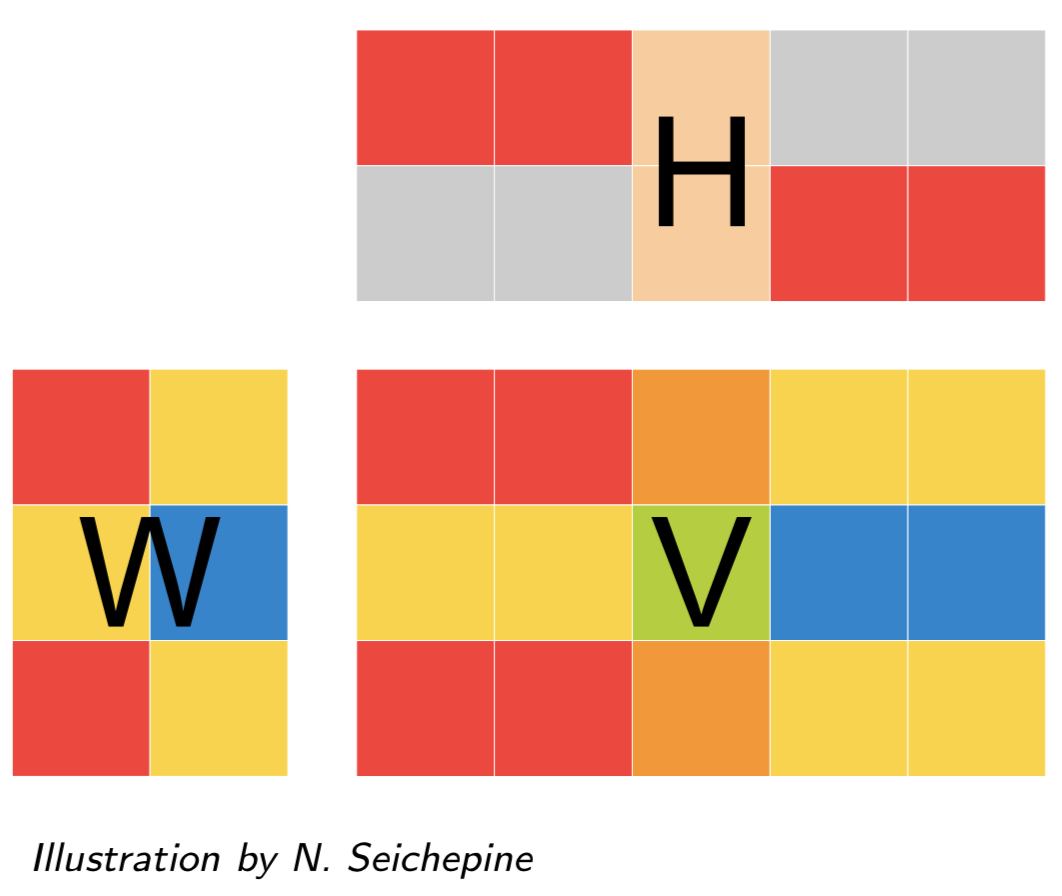
\includegraphics[scale=0.4]{rapport/images/Ch3_NMF1.png}
\end{center}
\caption{Factorisation NMF}
\end{figure}

\begin{equation*}
V \approx WH \\
\text{ avec }
W=[w_{fk}] \text{ tels que } w_{fk} \geq 0 \text{ et } \\
H=[h_{kn}] \text{ tels que } h_{kn} \geq 0.
\end{equation*}
Lors de cette factorisation des contraintes de positivité sont imposées afin de rendre les résultats interprétables d'un point de vue physique, ce qui constitue l'un des avantages de ces méthodes. On parle alors de Factorisation de matrices positives ou en anglais Non-Negative Matrix Factorization (NMF).


\subsubsection{Application}

La décomposition NMF est utilisée avec succès dans de nombreux contextes et domaines comme :

\begin{itemize}
    \item L'analyse de séquences de données temporelles,
    \item La séparation de sources,
    \item Le filtrage,
    \item Le clustering,
    \item etc. 
\end{itemize}

\paragraph{}
Dans le domaine audio, elle constitue l'état de l'art des packages de séparation de sources et de débruitage. Elle est également utilisée dans le domaine médical pour l'extraction de caractéristiques et le rejet d'artefacts dans les signaux d'encéphalogrammes \cite{Nguyen}

C'est pourquoi l'utilisation de cette méthode nous paraît adaptée pour résoudre notre problématique de détection des empreintes particulières.


Les publication les plus adaptées à notre contexte (à compléter) : 
\cite{JialiM}
\cite{Cheung}
